
%------------------------------------------------
% Semesterarbeit ESA
% 
% Autor:	Sandro Dallo sandro.dallo@students.ffhs.ch, Patrick Bösch patrick.boesch@students.ffhs.ch
%			Jonas Alder jonas.alder@students.ffhs.ch, Andy Villiger andy.villiger@students.ffhs.ch
% Datum:	17.09.2014
%
% Version:	1.0
%
%------------------------------------------------

%-- Preamble ------------------------------------
\documentclass[10pt,a4paper,twoside]{article}

%-- Nur für Debugging
%\usepackage{showframe}
\usepackage{float}
\usepackage{blindtext}
\usepackage{url} % Bibtext url
\usepackage[space]{grffile}

%-- Import packages -----------------------------
% Anpassung an deutsche Sprache
% Umlaute ----------------------------------------------------------------------
%   Umlaute/Sonderzeichen wie äüöß direkt im Quelltext verwenden (CodePage).
%   Erlaubt automatische Trennung von Worten mit Umlauten.
% ------------------------------------------------------------------------------
\usepackage[utf8]{inputenc}
\usepackage[T1]{fontenc}
\usepackage[ngerman]{babel}

% Code support
\usepackage{listings}

% Seitenränder und Zeilenabstände
\usepackage{geometry}
\usepackage{setspace}

% Schriften und Farben
\usepackage{color}
\usepackage{xcolor}
\usepackage{colortbl} % Für farbige Tabellen
\usepackage[default,osfigures,scale=1]{opensans} % Select font

% Textumgebungen
\usepackage{multicol} % Text in mehreren Kolumnen darstellen

% Tabellen
\usepackage{hhline}
\usepackage{array}
\usepackage{longtable}

% Floatbarrier 
\usepackage{placeins} 
% Hyperrefs und PDF Information
\usepackage{hyperref}
\usepackage{caption}
\usepackage{subcaption}

% Tabellen
\usepackage{booktabs}

% Inhaltsverzeichnis umbenennen
\usepackage{tocbibind}

% Listen
\usepackage[ampersand]{easylist} % Einfache Liste Umgebung
% http://en.wikibooks.org/wiki/LaTeX/List_Structures

% Kopf und Fusszeilen
\usepackage{fancyhdr}

% Grafiken und Textbausteine
\usepackage[absolute]{textpos} % Absolue Positionierung
%\usepackage[dvips,final]{graphicx} % Einbinden von JPG-Grafiken ermöglichen für
%dvi format
\usepackage[pdftex]{graphicx}
\usepackage{graphics} % keepaspectratio
\usepackage{floatflt} % zum Umfließen von Bildern
\graphicspath{{bilder/}} % hier liegen die Bilder des Dokuments

% Mathe
\usepackage{amsmath}
\usepackage{amssymb}

% Acronym Support
\usepackage[printonlyused]{acronym}
%-- Import Dokumenten Infos ---------------------
%----------------------------------------------------------
% Allgemeine Dokumenten Informationen wie Titel, Untertitel
% Autor, etc..
% gehören in dieses Dokumentenfragment.
%----------------------------------------------------------


\newcommand{\titel}{ESA - Proximety}
\newcommand{\untertitel}{Projektdokumentation}
\newcommand{\autor}{Jonas Alder, Patrick Bösch\\Sandro Dallo, Andy Villiger}
\newcommand{\comment}{FFHS Bsc Inf 2011}
\newcommand{\version}{0.1}
\newcommand{\datum}{17.09.2014}
\newcommand{\logo}{bilder/allgemein/logo.png}
%-- Import Seitenstil ---------------------------
% Setzen der Seitenränder
\geometry{top=30mm,left=30mm,right=30mm,bottom=35mm,a4paper}
\setlength{\marginparwidth}{20mm}

% Kein Einzug
\setlength{\parindent}{0cm} 

% Konfiguration für das textpos
\setlength{\TPHorizModule}{1mm}
\setlength{\TPVertModule}{\TPHorizModule}
\textblockorigin{0mm}{0mm}

% Kopf und Fusszeilen
\setlength{\headheight}{15.2pt}
\pagestyle{fancy}

% Hyperref
\hypersetup{
    bookmarks=false,         % show bookmarks bar?
    unicode=false,          % non-Latin characters in Acrobat’s bookmarks
    pdftoolbar=true,        % show Acrobat’s toolbar?
    pdfmenubar=true,        % show Acrobat’s menu?
    pdffitwindow=false,     % window fit to page when opened
    pdfstartview={FitH},    % fits the width of the page to the window
    pdftitle={\titel},    % title
    pdfauthor={\autor},     % author
    pdfsubject={\untertitel},   % subject of the document
    pdfcreator={LaTex},   % creator of the document
    pdfproducer={TeXEclipse}, % producer of the document
    %pdfkeywords={keyword1} {key2} {key3}, % list of keywords
    pdfnewwindow=true,      % links in new window
    colorlinks=true,       % false: boxed links; true: colored links
    linkcolor=black,          % color of internal links (change box color with linkbordercolor)
    citecolor=black,        % color of links to bibliography
    filecolor=black,      % color of file links
    urlcolor=black           % color of external links
}
%-- Import Definitions --------------------------
\definecolor{warning}{RGB}{244,250,164}
\definecolor{warning-line}{RGB}{231,244,66}
\definecolor{error}{RGB}{254,160,160}
\definecolor{error-line}{RGB}{254,56,56}
%-- Import Kopf und Fusszeilen ------------------
\fancyhf{} % Reset aktueller Style
%-- Header -----------------------
\fancyhead[LO,RE]{% 

\includegraphics[scale=0.25]{bilder/allgemein/logo.png}
}
\fancyhead[C]{% Header
\textit{\titel}
}
\fancyhead[LE,RO]{%
\textit{Seite \thepage}
}
\renewcommand{\headrule}
{
\hrule
\vspace{1mm}
}
%-- Footer -----------------------
\renewcommand\footrule{\
\hrule
\vspace{1mm}
}%
\fancyfoot[LO,RE]{% 
\small{\textit{\today}}
}
\fancyfoot[LE,RO]{%
\small{\textit{\autor}}
}
%-- Import Kommandos und Environments -----------
%----------------------------------------------------------
% Allgemeine Latex commands, enviroments etc...
% gehören in dieses Dokumentenfragment.
%----------------------------------------------------------
%-- Renew paragraph command -------------------------------
\makeatletter
\renewcommand\paragraph{%
   \@startsection{paragraph}{4}{0mm}%
      {-\baselineskip}%
      {.5\baselineskip}%
      {\normalfont\normalsize\bfseries}}
\makeatother
%-- Abbildungsverzeichnis ---------------------------------
\renewcommand{\listoffigures}{%
\begingroup
  \tocsection
  \tocfile{\listfigurename}{lof}
\endgroup}
%-- Abbildungsverzeichnis ---------------------------------
\renewcommand{\listoftables}{%
\begingroup
  \tocsection
  \tocfile{\listtablename}{lot}
\endgroup}
%-- Listings ---------------------------------------------
\renewcommand{\lstlistingname}{Code}
\renewcommand{\lstlistlistingname}{Codelistings}
\renewcommand{\lstlistoflistings}{%
\begingroup
  \tocsection
  \tocfile{\lstlistlistingname}{lol}
\endgroup}

%-- Aufgabe mit Trennlinie --------------------------------
\newcounter{cntaufgabe}
\newcounter{cntfrage}
\setcounter{cntfrage}{1}
\newcommand{\resetaufgabe}{%
\par
\vspace{10mm}
\leftskip=0cm
\setcounter{cntfrage}{1}
}
\newcommand{\aufgabe}[1]{%
\stepcounter{cntaufgabe}
\resetaufgabe
\vspace{2ex}
\begin{tabular}{ r p{0.8\textwidth} }
\textbf{\thecntaufgabe} &
\textbf{#1}
\end{tabular}
\vspace{1mm}
\hrule
\vspace{2ex}%
}
%-- Frage mit Trennlinie --------------------------------
\newcommand{\frage}[1]{%
\par
 \vspace{5mm}
\leftskip=1.4cm
\begin{tabular}{ r p{0.8\textwidth} }
\alph{cntfrage}) &
\textit{#1}
\end{tabular}
\vspace{1mm}
\par
\leftskip=2.35cm
\stepcounter{cntfrage}
}
%-- new paragraph ------------
\newcommand{\vpar}{
\par
\vspace{1ex}
}
%-- quick multicolumn ------
\newcommand{\mc}[1]{
	\multicolumn{2}{|p{0.49\textwidth}|}{#1}
}

%-- Import Tabellendefinitionen -----------
% Definieren von Tabellen und Boxes Umgebung
% UseCase Tables
\newenvironment{usecase}%
{%
\setlength{\tabcolsep}{5pt}
\setlist[itemize]{noitemsep,topsep=0pt,partopsep=0pt}
\setlist[enumerate]{noitemsep,topsep=0pt,partopsep=0pt}
%\renewcommand{\arraystretch}{2.5}
\centering
\begin{longtable}[H]{|l|p{9cm}|}
\arrayrulecolor{black}
\hline
}{%
\end{longtable}
}%
\newcommand{\ucElement}[2]{%
\textbf{#1} & \mbox{}\par\vspace{-\baselineskip}#2\\
\hline
}
% Tabellen definieren
\newenvironment{deftab}[3]%
{%
\setlength{\tabcolsep}{20pt}
\renewcommand{\arraystretch}{1.5}
\def\cap{#2}
\def\lab{#3}
\begin{table}[!htbp]
\footnotesize
\begin{center}
\begin{longtable}{#1}
}{%
\end{longtable}
\end{center}
\caption{\cap} % Text unter Tabelle
\label{table:\lab} % Referenz der Tabelle \ref{table:xyz}
\end{table}
\FloatBarrier % Sicherstellen das alles weitere nach der Tabelle kommt
}%
% -------------------------------------------------------
% Boxes
% Warnbox
\newsavebox{\wbox}
\newenvironment{warnbox}[1][]
  {%
   \setlength{\fboxsep}{8pt}
   \setlength{\fboxrule}{1pt}
   \footnotesize
   \newcommand\colboxcolor{#1}%
   \begin{lrbox}{\wbox}%
   \begin{minipage}[c]{0.9\textwidth}%   
 }{%
  \end{minipage}
  \end{lrbox}%
   \begin{center}
   \fcolorbox{warning-line}{warning}{\usebox{\wbox}}
\end{center}}
% Errorbox
\newsavebox{\ebox}
\newenvironment{errorbox}[1][]
  {%
   \setlength{\fboxsep}{8pt}
   \setlength{\fboxrule}{1pt}
   \footnotesize
   \newcommand\colboxcolor{#1}%
   \begin{lrbox}{\ebox}%
   \begin{minipage}[c]{0.9\textwidth}%
 }{%
  \end{minipage}
  \end{lrbox}%
   \begin{center}
   \fcolorbox{error-line}{error}{\usebox{\ebox}}
\end{center}}
%-- Tabellen ----------------------------------------------
\newcolumntype{+}{>{\global\let\currentrowstyle\relax}}
\newcolumntype{^}{>{\currentrowstyle}}
\newcommand{\rowstyle}[1]{\gdef\currentrowstyle{#1}%
#1\ignorespaces
}
\newcolumntype{L}[1]{>{\raggedright\arraybackslash}p{#1}} % linksbündig mit Breitenangabe
\newcolumntype{C}[1]{>{\centering\arraybackslash}p{#1}} % zentriert mit Breitenangabe
\newcolumntype{R}[1]{>{\raggedleft\arraybackslash}p{#1}} % rechtsbündig mit Breitenangabe
\newcommand{\ltab}{\raggedright\arraybackslash} % Tabellenabschnitt linksbündig
\newcommand{\ctab}{\centering\arraybackslash} % Tabellenabschnitt zentriert
\newcommand{\rtab}{\raggedleft\arraybackslash} % Tabellenabschnitt rechtsbündig
%-- Tabllenabstände
%\setlength{\tabcolsep}{10mm} % Column
\renewcommand{\arraystretch}{1.5} % Row
% -- Code Styling -------------------------------
\definecolor{lightgray}{RGB}{224,224,224}
\begin{document}
%-- Deckblatt -----------------------------------
\thispagestyle{empty}
\newgeometry{top=25mm,left=20mm,right=65mm,bottom=30mm} % Layout für Deckblatt
\begin{textblock}{1}(155,35)

\includegraphics[scale=0.25]{bilder/allgemein/deckblatt.png}
\end{textblock}
\begin{titlepage}
\hspace{\fill}
\vspace{30mm}
% Titel
\begin{center}
\Huge{\textbf{\titel}}\\[4ex]
\LARGE{\untertitel}\\[6ex]

\includegraphics[scale=0.2]{../02_Images/proximety.png}\\
\end{center}
\vspace{20mm}
% Autor, Kommentar, Logo etc 
\begin{flushright}

\includegraphics[scale=1]{bilder/allgemein/logo.png}\\[2ex]
\begin{Large}
\autor\\
\comment\\
Version \version\\
\datum\\
\end{Large}
\end{flushright}
\end{titlepage}
\restoregeometry % Aktuelles Seitelayout wiederherstellen
\newpage
% Dokumentenverlauf
\newpage
\section*{Dokumentenverlauf}
\begin{center}
	\begin{tabular}{  llp{9cm}l }
		\textbf{Version} & \textbf{Wer} & \textbf{Bemerkungen} & \textbf{Datum} \\\hline
		0.1 & DAL & Initialer Entwurf & 17.09.2014 \\
		0.2 & DAL & UseCase Diagramm hinzugefügt & 19.09.2014 \\
		0.3 & BOE & Kapitel Allgemeines ausformuliert & 21.09.2014 \\
		0.4 & BOE & GUI Prototypes Einleitung hinzugefügt, Flow Chart hinzugefügt und Fehler gemäss Rückmeldung Dozent korrigiert & 19.10.2014 \\
		0.5 & DAL & GUI Prototypes Variante 1 hinzugefügt, Korrekturen am Dokument vorgenommen & 19.10.2014 \\
		0.6 & ALO & GUI Prototypes Variante 2 und Vergleich hinzugefügt & 20.10.2014 \\
		0.7 & VIL & Kapitel Architektur eingefügt & 17.11.2014 \\
		0.8 & BOE & Architektur ergänzt und korrigiert & 17.11.2014 \\
	\end{tabular}
\end{center}
\newpage
%-- Inhaltsverzeichnis --------------------------
\setcounter{tocdepth}{5} % Tiefe des Inhaltsverzeichnis
\setcounter{secnumdepth}{5} % Nummerierungstiefe
\tableofcontents
\newpage 
%-- Allgemeines --------------------------
\section{Allgemeines}
\subsection{Einleitung}
%-- Anforderungen --------------------------
\section{Anforderungen}
\subsection{Funktional}
%-- Use Cases --------------------------
\subsubsection{Use Case Diagramm}
\begin{figure}[hp]
	\centering
		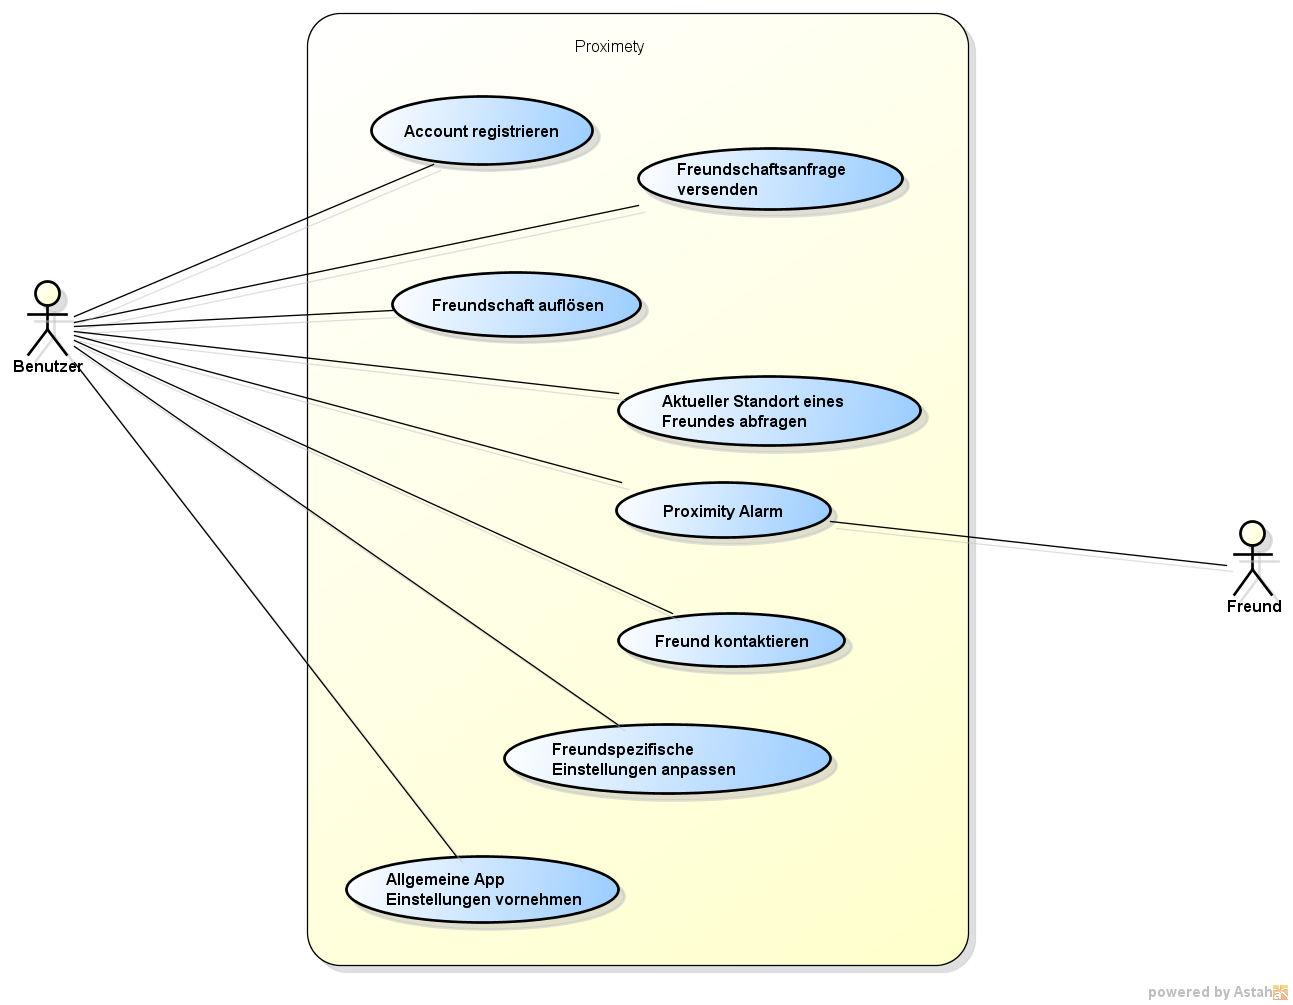
\includegraphics[scale=0.4]{BasicUseCaseDiagramm.png}
	\caption{Basis UseCase Diagramm}
	\label{fig:BasicUseCaseDiagramm}
\end{figure}
\FloatBarrier
% ------------------------------------------------------------------
\subsubsection{Use Case Beschreibungen}
% ------------------------------------------------------------------
\paragraph{UC01 - Account registrieren}
\begin{usecase}	
	\ucElement{ID}{UC01}
	\ucElement{Name}{Account registrieren}
	\ucElement{Kurzbeschreibung}{Der Benutzer registriert sich am System und erhält Logindaten.}
	\ucElement{Akteur}{Benutzer}
	\ucElement{Auslöser}{Der Akteur beginnt mit der Registrierung}
	\ucElement{Vorbedingungen}{App muss auf dem Gerät des Benutzers}
	\ucElement{Eingehende Informationen}{E-Mailadresse, Benutzername, Passwort}
	\ucElement{Ergebnis}{Registrierungsbestätigung}
	\ucElement{Nachbedingungen}{Benutzerkonto wurde erstellt}
	\ucElement{Ablauf}{%
		\begin{enumerate}
			\item Akteur startet Registrierungsprozess
			\item Akteur gibt E-Mailadresse und Passwort ein (inkl. Bestätigung)
			\item Akteur gibt Benutzernamen ein
			\item Akteur bestätigt die Registrierung.
		\end{enumerate}
		Es wird explizit darauf verzichtet eine aktivierungs E-Mail zu versenden.     
	}
	\ucElement{Alternativer Ablauf}{ %
				\begin{enumerate}
					\item[4a.]  Benutzername oder E-Mail werden bereits verwendet. Benutzer wird aufgefordert diese zu ändern.
				\end{enumerate}
		}
	\ucElement{Priorität}{Hoch}
	\ucElement{Aufwand}{?}
	\ucElement{Status}{Offen}
	\ucElement{Änderungshistorie}{?}
\end{usecase}
% ------------------------------------------------------------------
\paragraph{UC02 - Freundschaftsanfrage versenden}
\begin{usecase}	
	\ucElement{ID}{UC02}
	\ucElement{Name}{Freundschaftsanfrage versenden}
	\ucElement{Kurzbeschreibung}{Der Benutzer sendet eine Anfrage an einen anderen Benutzer um ihn seiner persönlichen Freundesliste hinzu zufügen.}
	\ucElement{Akteur}{Benutzer}
	\ucElement{Auslöser}{Der Akteur beginnt mit der Suche nach einem Freund}
	\ucElement{Vorbedingungen}{Benutzer besitzt einen Account}
	\ucElement{Eingehende Informationen}{E-Mailadresse oder Benutzername eines Benutzers}
	\ucElement{Ergebnis}{Freundesanfrage an anderen Benutzer}
	\ucElement{Nachbedingungen}{}
	\ucElement{Ablauf}{%
		\begin{enumerate}
			\item Akteur sucht einen Benutzer anhand Benutzername oder E-Mail
			\item Akteur wählt Benutzer aus Ergebnisliste aus um eine Anfrage zu versenden
			\item Angefragter Benutzer entscheidet über die Anfrage (Annahme/Ablehnen)
			\item Akteur wird über das Ergebnis informiert.
		\end{enumerate}    
	}
	\ucElement{Alternativer Ablauf}{}
	\ucElement{Priorität}{Hoch}
	\ucElement{Aufwand}{?}
	\ucElement{Status}{Offen}
	\ucElement{Änderungshistorie}{?}
\end{usecase}
% ------------------------------------------------------------------
\paragraph{UC03 - Freundschaft auflösen}
\begin{usecase}	
	\ucElement{ID}{UC03}
	\ucElement{Name}{Freundschaft auflösen}
	\ucElement{Kurzbeschreibung}{Der Benutzer entfernt einen anderen Benutzer von seiner Freundesliste}
	\ucElement{Akteur}{Benutzer}
	\ucElement{Auslöser}{Der Akteur möchte einen Freund aus seiner Liste entfernen.}
	\ucElement{Vorbedingungen}{ %
		\begin{itemize}
			\item Benutzer besitzt einen Account
			\item Benutzer besitzt mind. einen Freund			
		\end{itemize}
		}
	\ucElement{Eingehende Informationen}{Der zu entfernende Freund}
	\ucElement{Ergebnis}{Benachrichtigung an beide Benutzer}
	\ucElement{Nachbedingungen}{Akteur und ausgewählter Benutzer sind keine Freunde mehr.}
	\ucElement{Ablauf}{%
		\begin{enumerate}
			\item Akteur sucht einen Benutzer in seiner Freundesliste			
			\item Akteur wählt Benutzer aus und wählt “Freund entfernen”
			\item Akteur bestätigt seine Wahl (Annahme/Ablehnen)
			\item Beide Benutzer werden über das Ereignis informiert
		\end{enumerate}    
	}
	\ucElement{Alternativer Ablauf}{}
	\ucElement{Priorität}{Mittel}
	\ucElement{Aufwand}{?}
	\ucElement{Status}{Offen}
	\ucElement{Änderungshistorie}{?}	
\end{usecase}
% ------------------------------------------------------------------
\paragraph{UC04 - Aktueller Standort eines Freundes abfragen}
\begin{usecase}	
	\ucElement{ID}{UC04}
	\ucElement{Name}{Aktueller Standort eines Freundes abfragen}
	\ucElement{Kurzbeschreibung}{Der Benutzer fragt den aktuellen Standort eines Freundes ab. Dieser wird auf einer Karte angezeigt}
	\ucElement{Akteur}{Benutzer}
	\ucElement{Auslöser}{Der Akteur möchte einen Freund lokalisieren.}
	\ucElement{Vorbedingungen}{ %
		\begin{itemize}
			\item Benutzer besitzt einen Account
			\item Benutzer besitzt mind. einen Freund			
		\end{itemize}
	}
	\ucElement{Eingehende Informationen}{Der zu lokalisierende Freund}
	\ucElement{Ergebnis}{Standort des Freundes}
	\ucElement{Nachbedingungen}{}
	\ucElement{Ablauf}{%
		\begin{enumerate}
			\item Akteur sucht einen Benutzer in seiner Freundesliste			
			\item Akteur wählt Benutzer aus und wählt “Freund lokalisieren”
			\item Aktueller Standort wird von Freund abgerufen und auf einer Karte dargestellt.
		\end{enumerate}    
	}
	\ucElement{Alternativer Ablauf}{ %
		\begin{enumerate}
			\item[3a.] Standort kann nicht abgerufen werden: Entsprechende Fehlermeldung wird angezeigt. 
		\end{enumerate}
		}
	\ucElement{Priorität}{Hoch}
	\ucElement{Aufwand}{?}
	\ucElement{Status}{Offen}
	\ucElement{Änderungshistorie}{?}
\end{usecase}
% ------------------------------------------------------------------
\paragraph{UC05 - Proximity Alarm}
\begin{usecase}	
	\ucElement{ID}{UC05}
	\ucElement{Name}{Proximity Alarm}
	\ucElement{Kurzbeschreibung}{Benachrichtigung falls sich zwei Benutzer in definierter (oder weniger) Distanz zueinander befinden.}
	\ucElement{Akteur}{System}
	\ucElement{Auslöser}{System ermittelt Distanz zwischen Benutzern unter definiertem Schwellwert.}
	\ucElement{Vorbedingungen}{ %
		\begin{itemize}
			\item Beide Benutzer sind Freunde
			\item Aktueller Standort von beiden Benutzern bekannt
			\item Proximity Alarm für Freund aktiviert			
		\end{itemize}
	}
	\ucElement{Eingehende Informationen}{Standort der Benutzer}
	\ucElement{Ergebnis}{Benachrichtigung der beiden Benutzer}
	\ucElement{Nachbedingungen}{}
	\ucElement{Ablauf}{%
		\begin{enumerate}
			\item System prüft periodisch die Distanz zwischen Freunden			
			\item System versendet Benachrichtigung an die Benutzer
		\end{enumerate}    
	}
	\ucElement{Alternativer Ablauf}{}
	\ucElement{Priorität}{Hoch}
	\ucElement{Aufwand}{?}
	\ucElement{Status}{Offen}
	\ucElement{Änderungshistorie}{?}
\end{usecase}
% ------------------------------------------------------------------
\paragraph{UC06 - Freund kontaktieren}
\begin{usecase}	
	\ucElement{ID}{UC06}
	\ucElement{Name}{Freund kontaktieren}
	\ucElement{Kurzbeschreibung}{Benutzer kann einen Freund aus der App mit dritt Apps kontaktieren}
	\ucElement{Akteur}{Benutzer}
	\ucElement{Auslöser}{Benutzer möchte Freund kontaktieren}
	\ucElement{Vorbedingungen}{Beide Benutzer sind Freunde}
	\ucElement{Eingehende Informationen}{E-Mail des Freundes (z.Z. keine weiteren Kontaktinformationen vorhanden)}
	\ucElement{Ergebnis}{Dritt-App wird mit Kontaktinformationen (E-Mail) gestartet}
	\ucElement{Nachbedingungen}{}
	\ucElement{Ablauf}{%
		\begin{enumerate}
			\item Akteur sucht einen Benutzer in seiner Freundesliste			
			\item Benutzer wählt Kontakt App aus (z.B. Gmail)
			\item Dritt-App wird gestartet
		\end{enumerate}    
	}
	\ucElement{Alternativer Ablauf}{}
	\ucElement{Priorität}{Tief}
	\ucElement{Aufwand}{?}
	\ucElement{Status}{Offen}
	\ucElement{Änderungshistorie}{?}
\end{usecase}
% ------------------------------------------------------------------
\paragraph{UC07 - Freund-Spezifische Einstellungen anpassen}
\begin{usecase}	
\ucElement{ID}{UC07}
\ucElement{Name}{Freund-Spezifische Einstellungen anpassen}
\ucElement{Kurzbeschreibung}{Benutzer kann für jeden Freund Einstellungen anpassen (Tracking ein/aus, Distanz)}
\ucElement{Akteur}{Benutzer}
\ucElement{Auslöser}{Benutzer möchte Einstellungen ändern}
\ucElement{Vorbedingungen}{Beide Benutzer sind Freunde}
\ucElement{Eingehende Informationen}{Gewünschte Einstellungen}
\ucElement{Ergebnis}{Einstellungen sind angepasst}
\ucElement{Nachbedingungen}{}
\ucElement{Ablauf}{%
	\begin{enumerate}
		\item Akteur sucht einen Benutzer in seiner Freundesliste
		\item Benutzer ändert Einstellungen (Tracking ein/aus, Distanz)
		\item Benutzer bestätigt Eingaben
	\end{enumerate}       
}
\ucElement{Alternativer Ablauf}{}
\ucElement{Priorität}{Mittel}
\ucElement{Aufwand}{?}
\ucElement{Status}{Offen}
\ucElement{Änderungshistorie}{?}
\end{usecase}
% ------------------------------------------------------------------
\paragraph{UC08 - Allgemeine App Einstellungen vornehmen}
\begin{usecase}	
	\ucElement{ID}{UC08}
	\ucElement{Name}{Allgemeine App Einstellungen vornehmen}
	\ucElement{Kurzbeschreibung}{Der Benutzer kann allgemeine Einstellungen an der App vornehmen}
	\ucElement{Akteur}{Benutzer}
	\ucElement{Auslöser}{Der Akteur möchte Einstellungen ändern}
	\ucElement{Vorbedingungen}{ Benutzer besitzt einen Account}
	\ucElement{Eingehende Informationen}{}
	\ucElement{Ergebnis}{Einstellungen aktualisiert und gespeichert}
	\ucElement{Nachbedingungen}{}
	\ucElement{Ablauf}{%
		\begin{enumerate}
			\item Akteur wählt in der Naviagtion “Einstellungen” aus			
			\item Akteur kann Einstllungen anpassen (Standard Distanz für Alarm, Alarm Ton/Typ)
			\item Akteur bestätigt seine Einstellungen
		\end{enumerate}    
	}
	\ucElement{Alternativer Ablauf}{}
	\ucElement{Priorität}{Mittel}
	\ucElement{Aufwand}{?}
	\ucElement{Status}{Offen}
	\ucElement{Änderungshistorie}{?}
\end{usecase}

\section{GUI Prototypes}
\subsection{Einleitung}
Das GUI vom Proximety ist so aufgebaut, dass nur die für den aktuellen Context unerlässlichen Informationen dargestellt werden. So wird sichergestellt, dass der Benutzer nicht durch Informationen verwirrt wird, welche er für die aktuelle Aktion nicht gebrauchen kann.

Durch das Betätigen des Zurück-Knopfes kommt man im Applikationsfluss zurück auf die letzte Maske. Sollte sich der Benutzer auf dem Main Screen befinden, löst ein Drücken des Zurück-Knopfes das Schliessen der Applikation aus. 

Eingaben des Benutzers werden immer auf die Gültigkeit überprüft und mit einer Hinweis-Meldung (Snackbar / Toast) behandelt. Ein erfolgreiches vorwärts gerichtetes Verlassen der Screens ist erst möglich, wenn alle Eingaben gültig sind. Zusätzlich zur Meldung wird noch das Eingabe-Feld markiert, in welchem der Fehler aufgetreten ist.

Im den Flow Charts wird der Fluss der Applikation durch die einzelnen Masken visualisiert.
\subsection{Variante 1}
\subsection{Variante 1}
%\newcommand{\var1path}[1]{../02\_Images/gui\_variante\_1/{#1}}
%\newcommand{\guivarone}[1]{\detokenize{../02_Images/gui_variante_1/#1}}
\begin{figure}
	\centering
	\begin{subfigure}[b]{0.3\textwidth}
		%\includegraphics[width=\textwidth]{\guivarone{initialer_screen.png}}
		\caption{A gull}
		\label{fig:gull}
	\end{subfigure}%
	~ %add desired spacing between images, e. g. ~, \quad, \qquad, \hfill etc.
	%(or a blank line to force the subfigure onto a new line)
	\begin{subfigure}[b]{0.3\textwidth}
		%\includegraphics[width=\textwidth]{\guivarone{register_screen.png}}
		\caption{A tiger}
		\label{fig:tiger}
	\end{subfigure}
\end{figure}
\def\blabla{\detokenize{../02_Images/gui_variante_1/}}
\blabla
%\guivarone{initialer_screen.png}\par
\includegraphics[scale=0.5,width=\textwidth]{\protect\blabla{initialer_screen.png}}

\newpage
\subsection{Variante 2}
Der allgemeine Ablauf der Anwendung kann in der Abbildung~\ref{fig:ProximetyUIFlow2} entnommen werden. Anschliessend folgen alle bisher definierten Fenster der Variante 2.

\def\guivarone{bilder/guivariante2/}
\FloatBarrier
\begin{figure}[hp]
	\centering
	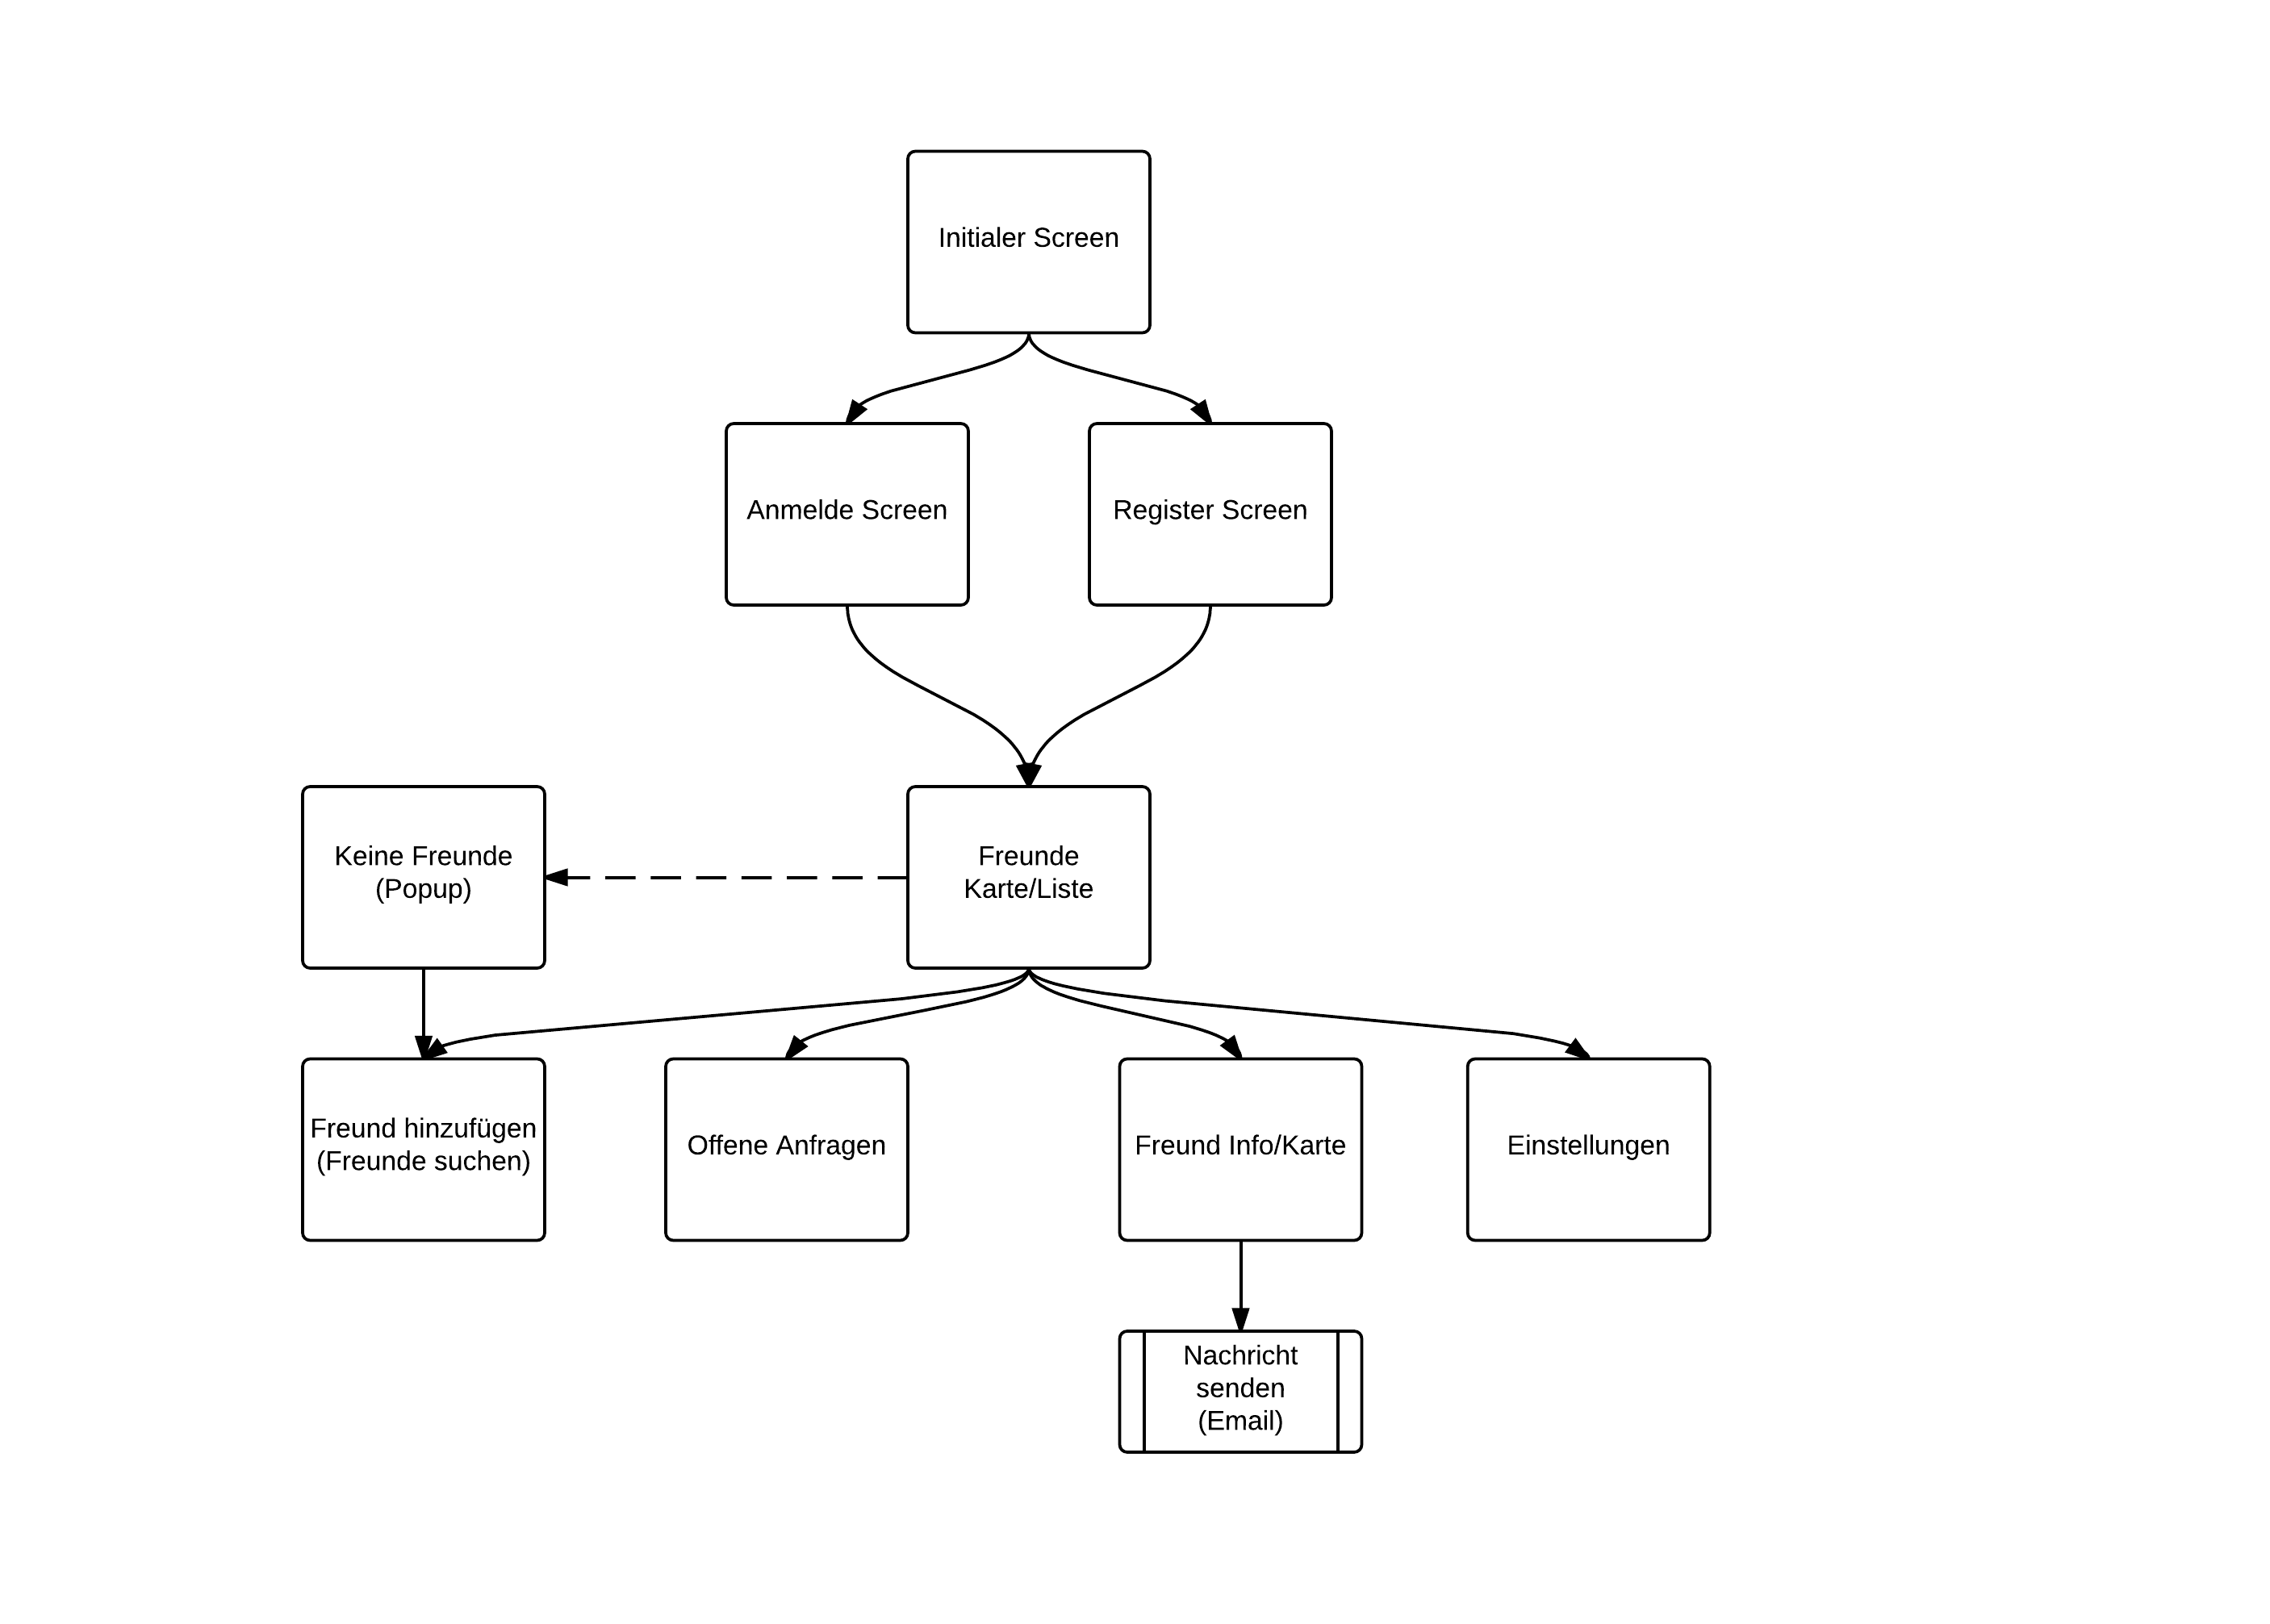
\includegraphics[scale=0.18]{ProximetyUIFlow2.png}
	\caption{Design Flow Diagramm}
	\label{fig:ProximetyUIFlow2}
\end{figure}
\FloatBarrier
\begin{figure}[H]
	\centering
	\begin{subfigure}[h]{0.3\textwidth}
		\includegraphics[width=1\textwidth]{\guivarone{Initialscreen.png}}
		\caption{Initiales Fenster}
		\label{fig:initscreentwo}
	\end{subfigure}%
	\qquad %add desired spacing between images, e. g. ~, \quad, \qquad, \hfill etc.
	%(or a blank line to force the subfigure onto a new line)
	\begin{subfigure}[h]{0.3\textwidth}
		\includegraphics[width=1\textwidth]{\guivarone{Registrieren.png}}
		\caption{Registrierungsfenster}
		\label{fig:registerscreentwo}
	\end{subfigure}
	\caption{Initialer und Registrierungsfenster}
\end{figure}
\begin{figure}[H]
	\centering
	\begin{subfigure}[h]{0.3\textwidth}
		\includegraphics[width=1\textwidth]{\guivarone{Anmelden.png}}
		\caption{Anmeldung}
		\label{fig:logintwo}
	\end{subfigure}%
	\qquad %add desired spacing between images, e. g. ~, \quad, \qquad, \hfill etc.
	%(or a blank line to force the subfigure onto a new line)
	\begin{subfigure}[h]{0.3\textwidth}
		\includegraphics[width=1\textwidth]{\guivarone{Leere Freundesliste.png}}
		\caption{Keine Kontakte}
		\label{fig:mainempty}
	\end{subfigure}
	\caption{Anmeldungs- und Hauptfenster (Ohne Kontakte)}
\end{figure}
\begin{figure}[H]
	\centering
	\begin{subfigure}[h]{0.3\textwidth}
		\includegraphics[width=1\textwidth]{\guivarone{Freunde - Liste.png}}
		\caption{Hauptfenster (Liste)}
		\label{fig:mainlist}
	\end{subfigure}%
	\qquad %add desired spacing between images, e. g. ~, \quad, \qquad, \hfill etc.
	%(or a blank line to force the subfigure onto a new line)
	\begin{subfigure}[h]{0.3\textwidth}
		\includegraphics[width=1\textwidth]{\guivarone{Freunde - Karte.png}}
		\caption{Hauptfenster (Karte)}
		\label{fig:mainmap}
	\end{subfigure}
	\caption{Hauptfenster in Listen- und Kartenansicht }
\end{figure}
\begin{figure}[H]
	\centering
	\begin{subfigure}[h]{0.3\textwidth}
		\includegraphics[width=1\textwidth]{\guivarone{Offene Anfragen.png}}
		\caption{Offene Anfragen}
		\label{fig:openrequests}
	\end{subfigure}%
	\qquad %add desired spacing between images, e. g. ~, \quad, \qquad, \hfill etc.
	%(or a blank line to force the subfigure onto a new line)
	\begin{subfigure}[h]{0.3\textwidth}
		\includegraphics[width=1\textwidth]{\guivarone{Freund hinzufuegen.png}}
		\caption{Freund hinzufügen}
		\label{fig:addfriend}
	\end{subfigure}
	\caption{Freundschatsanfragen stellen und beantworten }
\end{figure}
\begin{figure}[H]
	\centering
	\begin{subfigure}[h]{0.3\textwidth}
		\includegraphics[width=1\textwidth]{\guivarone{Freund - Details.png}}
		\caption{Freund Details}
		\label{fig:frienddetails}
	\end{subfigure}%
	\qquad %add desired spacing between images, e. g. ~, \quad, \qquad, \hfill etc.
	%(or a blank line to force the subfigure onto a new line)
	\begin{subfigure}[h]{0.3\textwidth}
		\includegraphics[width=1\textwidth]{\guivarone{Freund - Karte.png}}
		\caption{Freund Karte}
		\label{fig:friendmap}
	\end{subfigure}
	\caption{Detail- und Kartenansicht für Freund}
\end{figure}
\begin{figure}[H]
	\centering
	\begin{subfigure}[h]{0.3\textwidth}
		\includegraphics[width=1\textwidth]{\guivarone{Menu.png}}
		\caption{Menu}
		\label{fig:menu}
	\end{subfigure}%
	\qquad %add desired spacing between images, e. g. ~, \quad, \qquad, \hfill etc.
	%(or a blank line to force the subfigure onto a new line)
	\begin{subfigure}[h]{0.3\textwidth}
		\includegraphics[width=1\textwidth]{\guivarone{Notification - Alarm.png}}
		\caption{Benachrichtigung}
		\label{fig:loginscreenone}
	\end{subfigure}
	\caption{Menu und Benachrichtigung }
\end{figure}
\newpage
\subsection{Vergleich und Entscheid}
Da es das Ziel des Designs war, dass die Screens mit möglichst wenig Informationen und Elementen - sprich schlicht - daher kommen, haben wir uns für die zweite Variante entschieden.

Des Weiteren ist die Navigation im zweiten Vorschlag viel einfacher, da die Anzahl der Screens reduziert wurde. Für den Benutzer ist es so einfacher sich in der Applikation zu Recht zu finden. Das Menu wird im zweiten Vorschlag von jeder Maske mit einem Wisch zu erreichen sein – was den Android Konventionen entspricht und der Simplifizierung des Programms beiträgt.

Auch sticht sofort ins Auge, dass der Aufbau der einzelnen Masken dem "Material Design" von Android Lollipop (Android 5.0) und daher dem aktuellen Trend entspricht.
\newpage
\section{Architektur}
\subsubsection{Klassendiagramm App}
\begin{figure}[H]
	\centering
		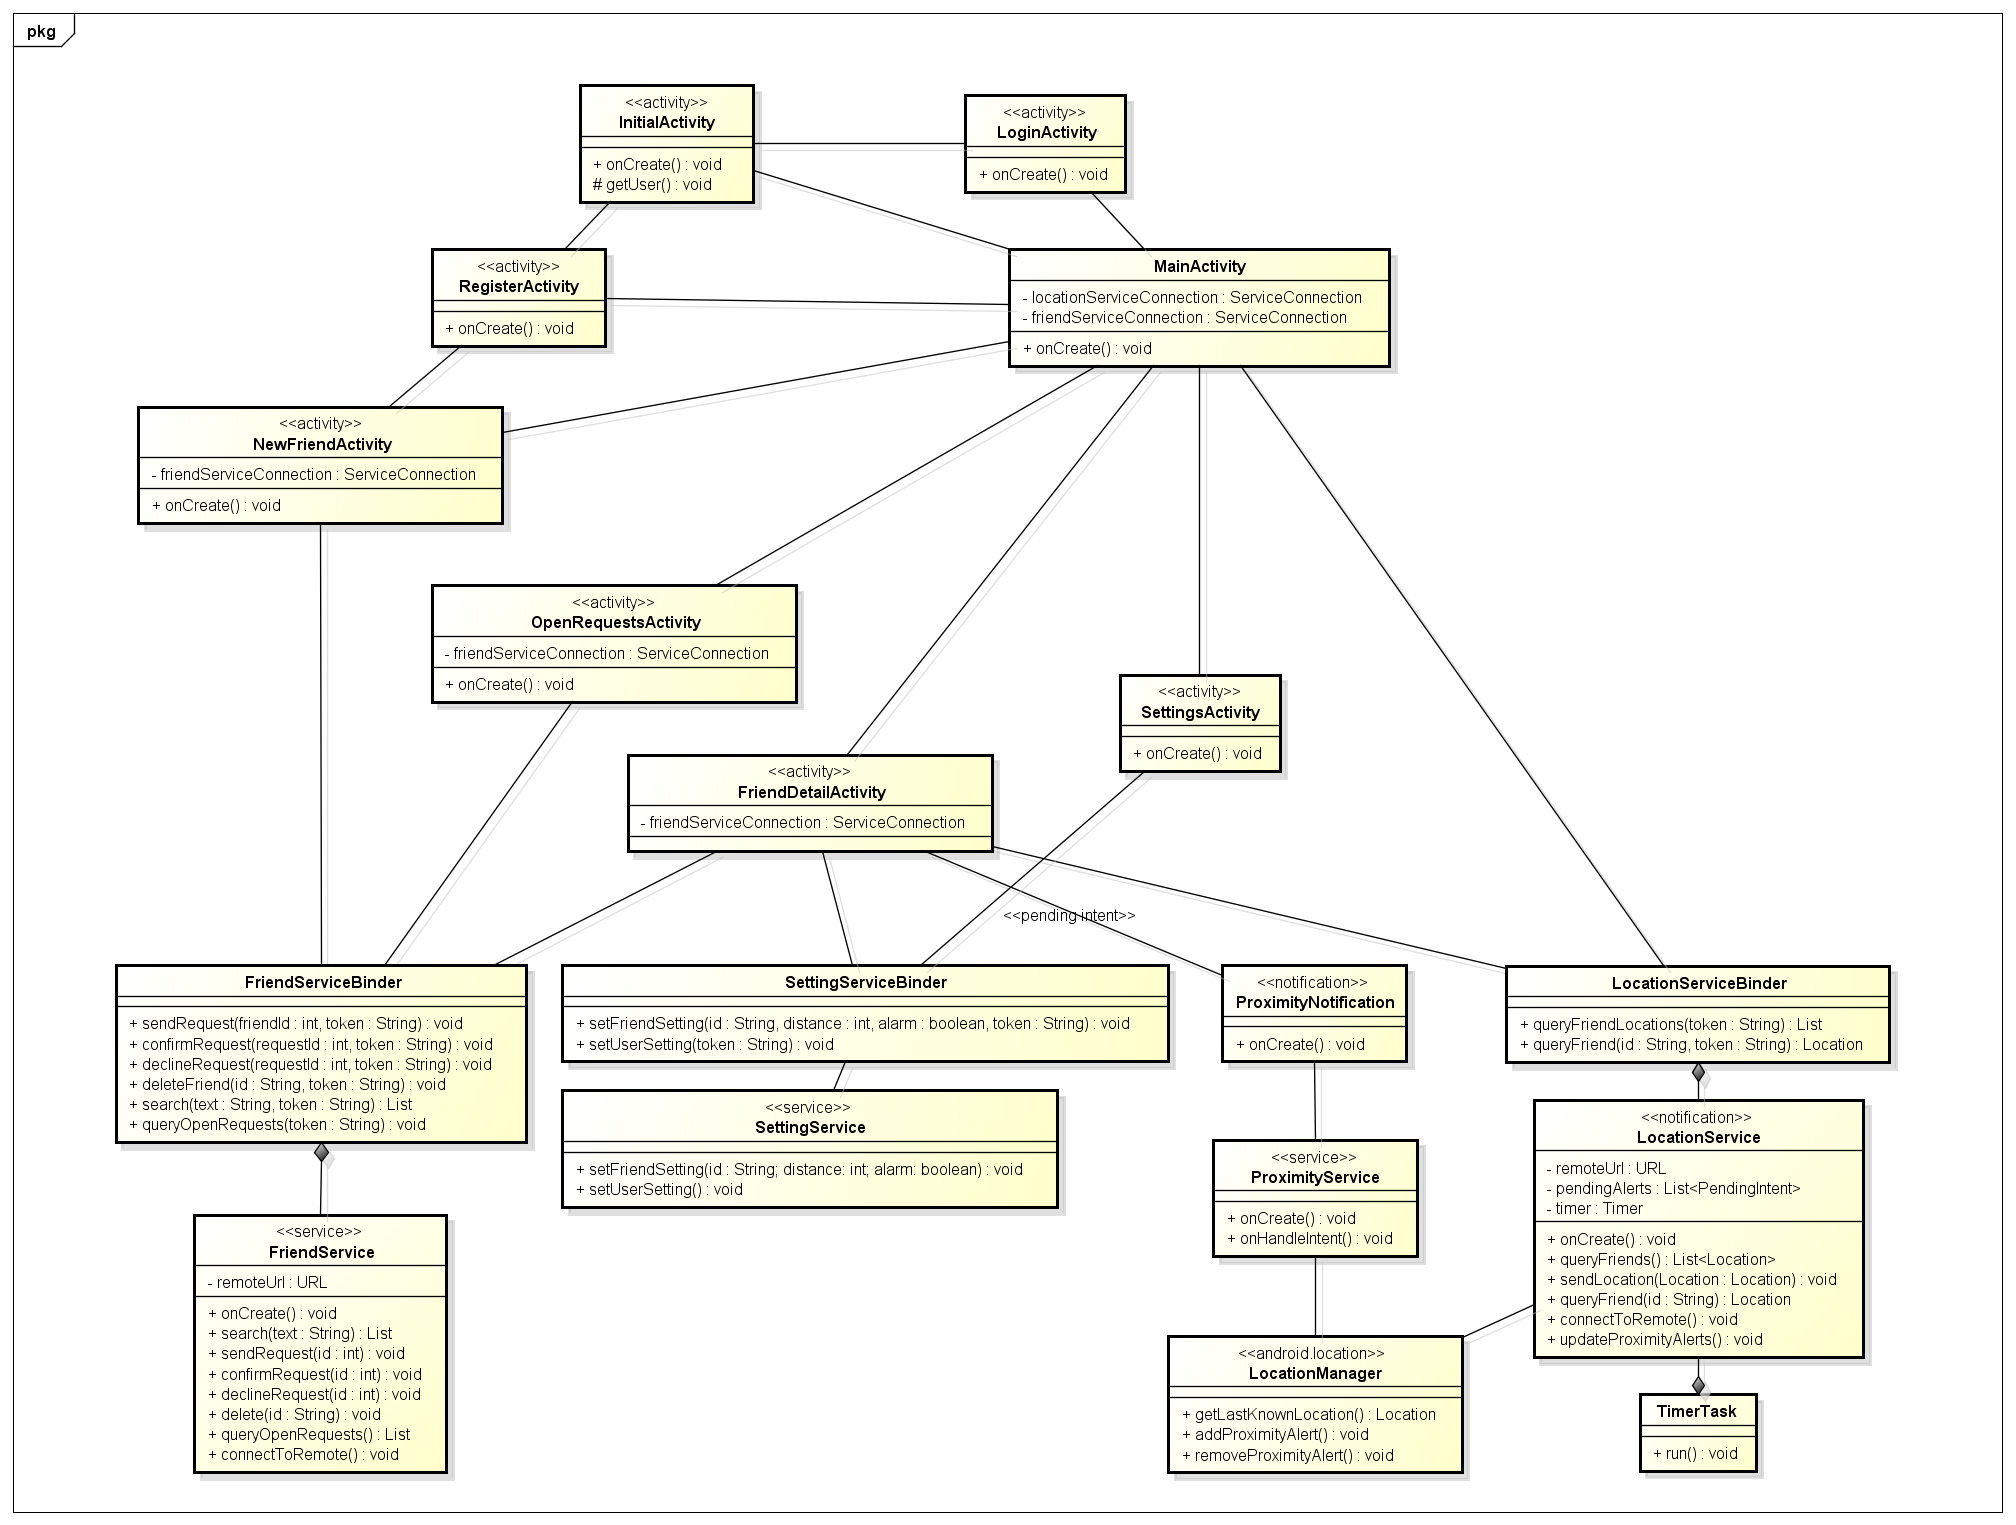
\includegraphics[width=\textwidth]{architektur/Proximety_Classes}
	\caption{Klassendiagramm der App}
	\label{fig:Proximety_Classes}
\end{figure}
\FloatBarrier



\pagebreak
\subsubsection{Klassendiagramm Server}
\begin{figure}[H]
	\centering
		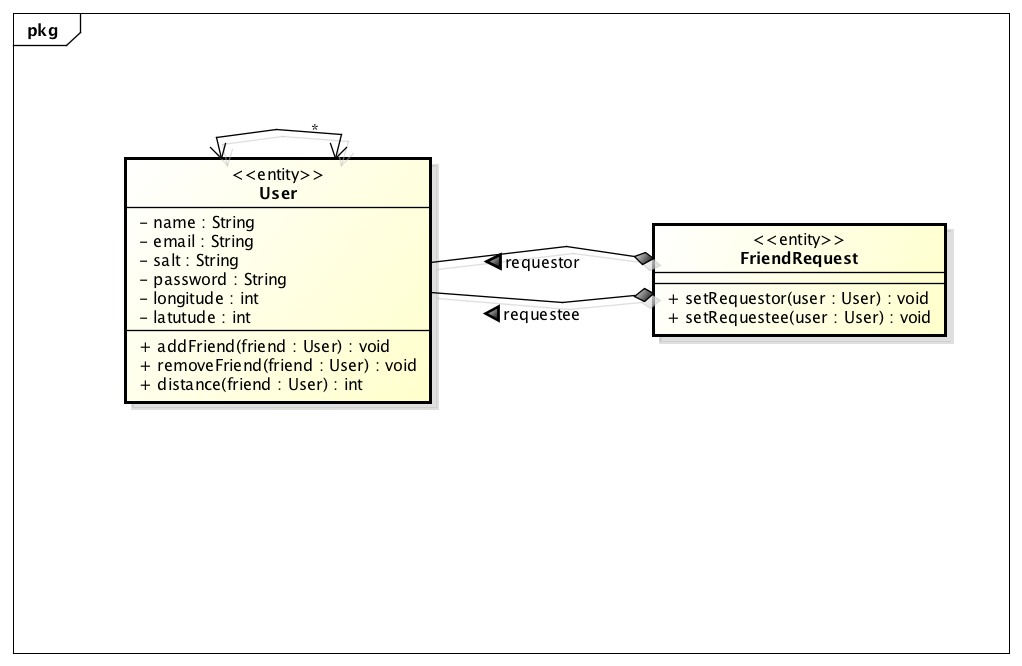
\includegraphics[width=\textwidth]{architektur/Proximety_Server_Classes}
	\caption{Klassendiagramm des Server}
	\label{fig:Proximety_Server_Classes}
\end{figure}
\FloatBarrier



\pagebreak
\subsubsection{Sequenzdiagramm Startup-Sequenz}
\begin{figure}[H]
	\centering
		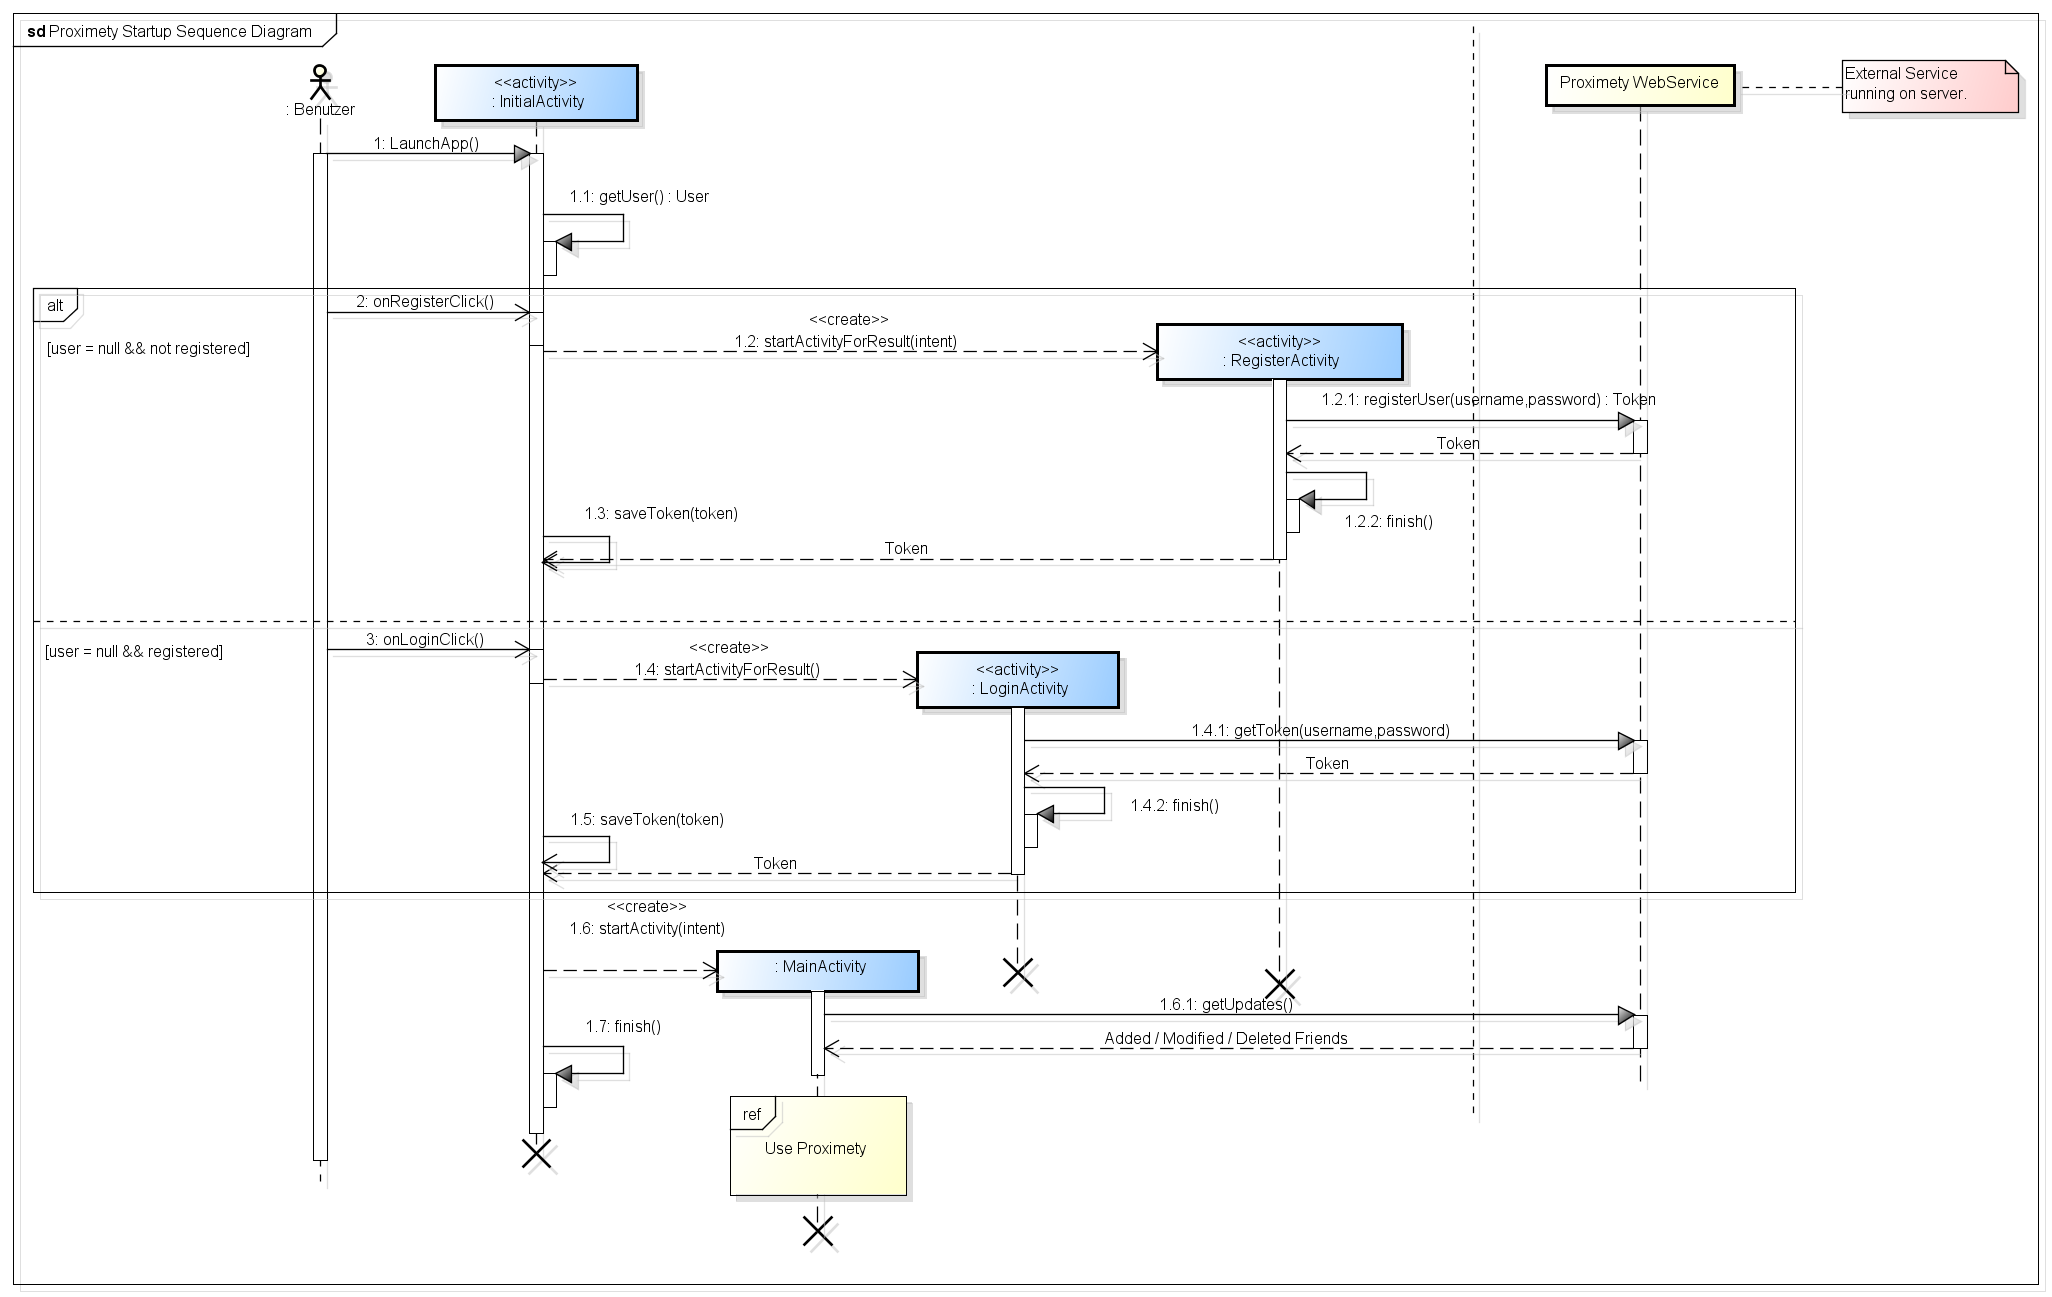
\includegraphics[width=\textwidth]{architektur/Proximety_Startup_Sequence_Diagram}
	\caption{Sequenzdiagramm Startup-Sequenz}
	\label{fig:Proximety_Startup_Sequence_Diagram}
\end{figure}
\FloatBarrier



\pagebreak
\subsubsection{Sequenzdiagramm Account registrieren}
\begin{figure}[H]
	\centering
		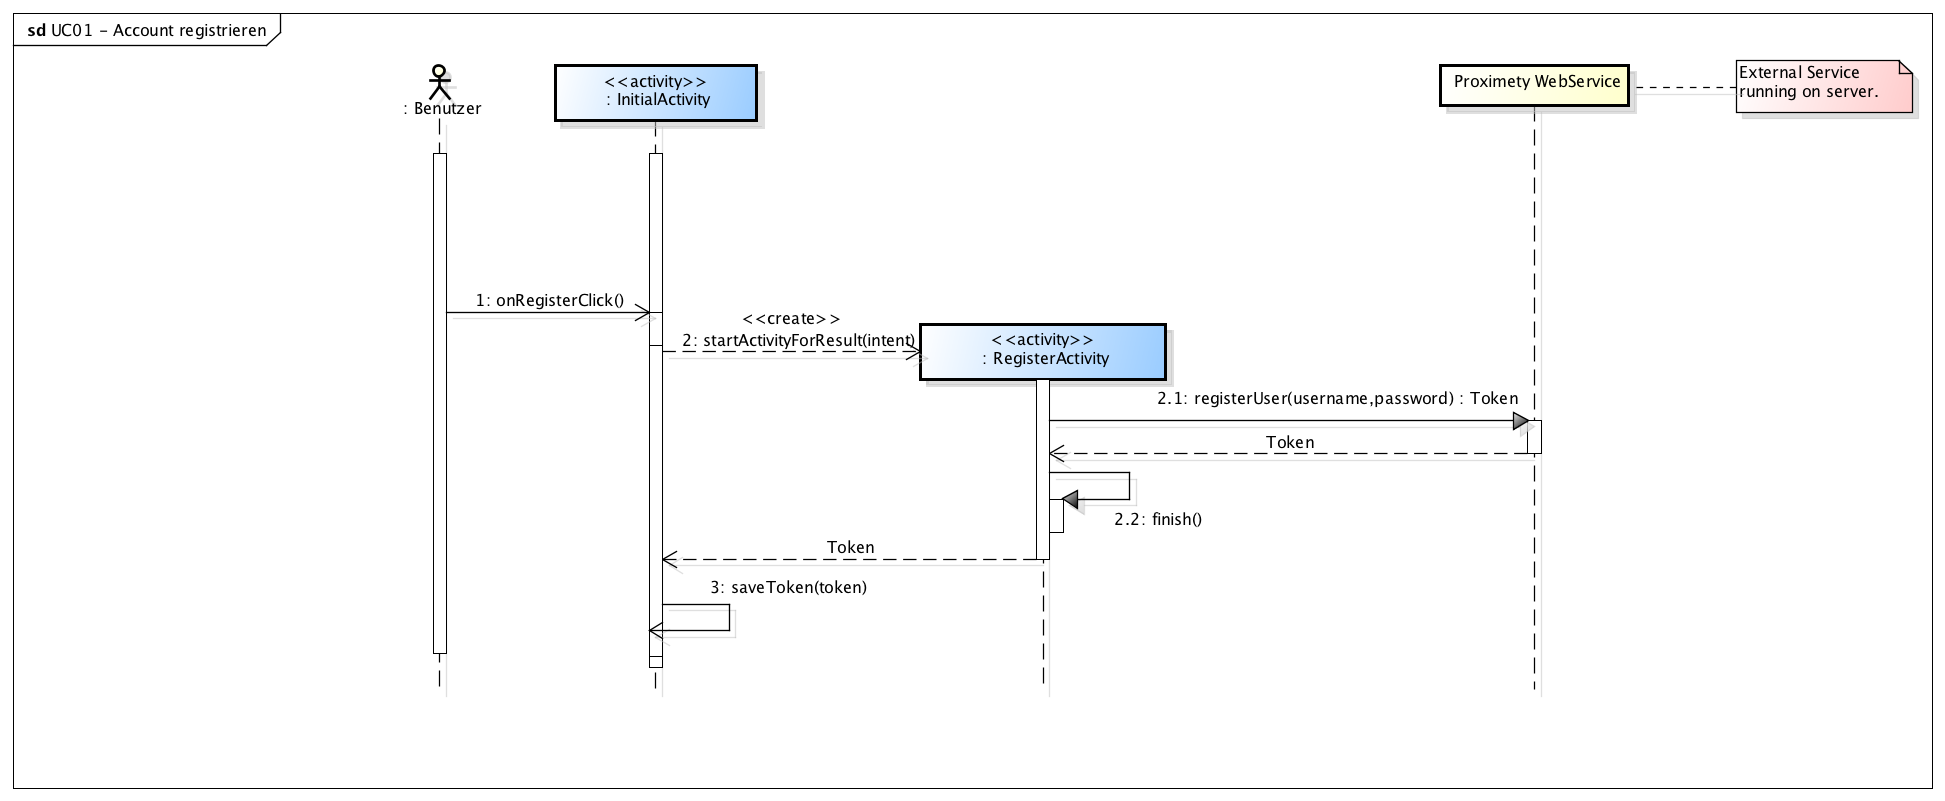
\includegraphics[width=\textwidth]{architektur/UC01_Account_registrieren}
	\caption{Sequenzdiagramm Account registrieren}
	\label{fig:UC01_Account_registrieren}
\end{figure}
\FloatBarrier



\pagebreak
\subsubsection{Sequenzdiagramm Freundschaftsanfrage versenden}
\begin{figure}[H]
	\centering
		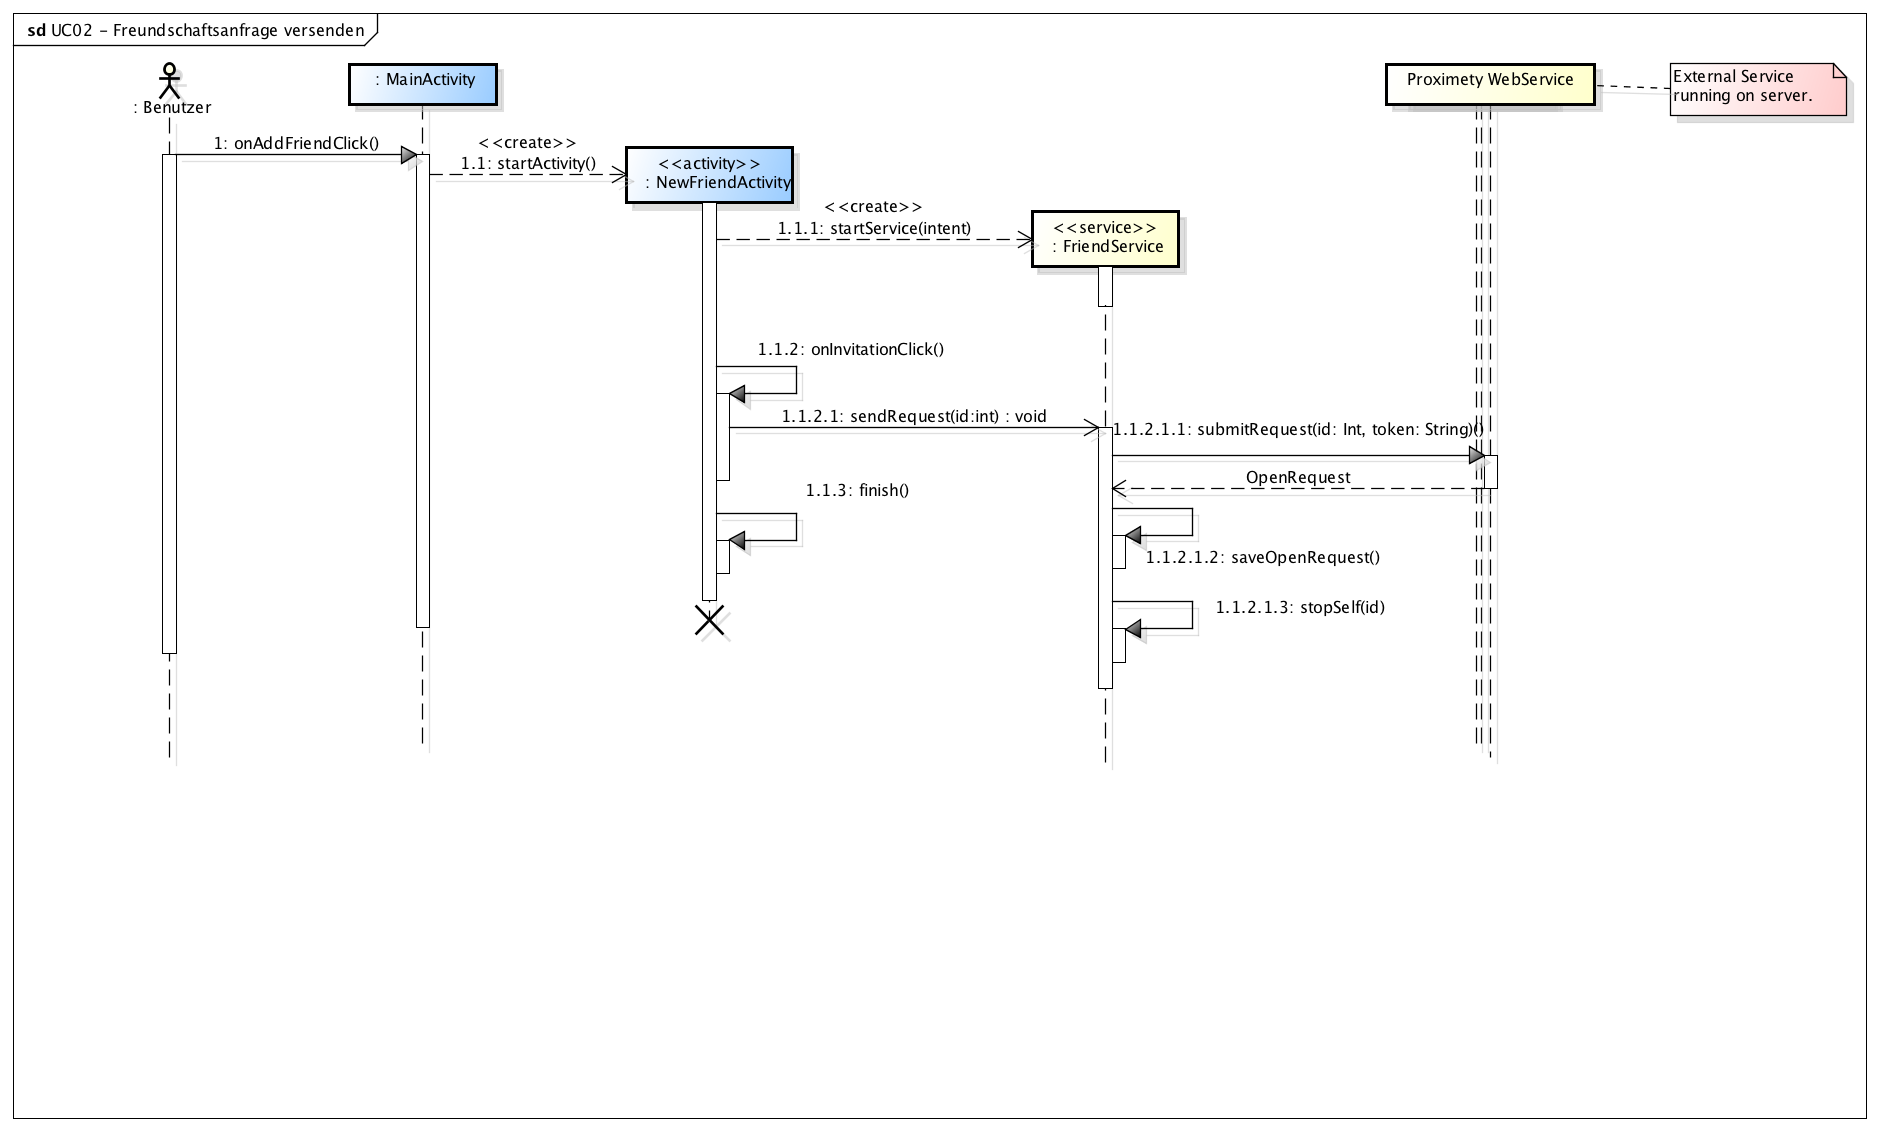
\includegraphics[width=\textwidth]{architektur/UC02_Freundschaftsanfrage_versenden}
	\caption{Sequenzdiagramm Freundschaftsanfrage versenden}
	\label{fig:UC02_Freundschaftsanfrage_versenden}
\end{figure}
\FloatBarrier



\pagebreak
\subsubsection{Sequenzdiagramm Freundschaft aufloesen}
\begin{figure}[H]
	\centering
		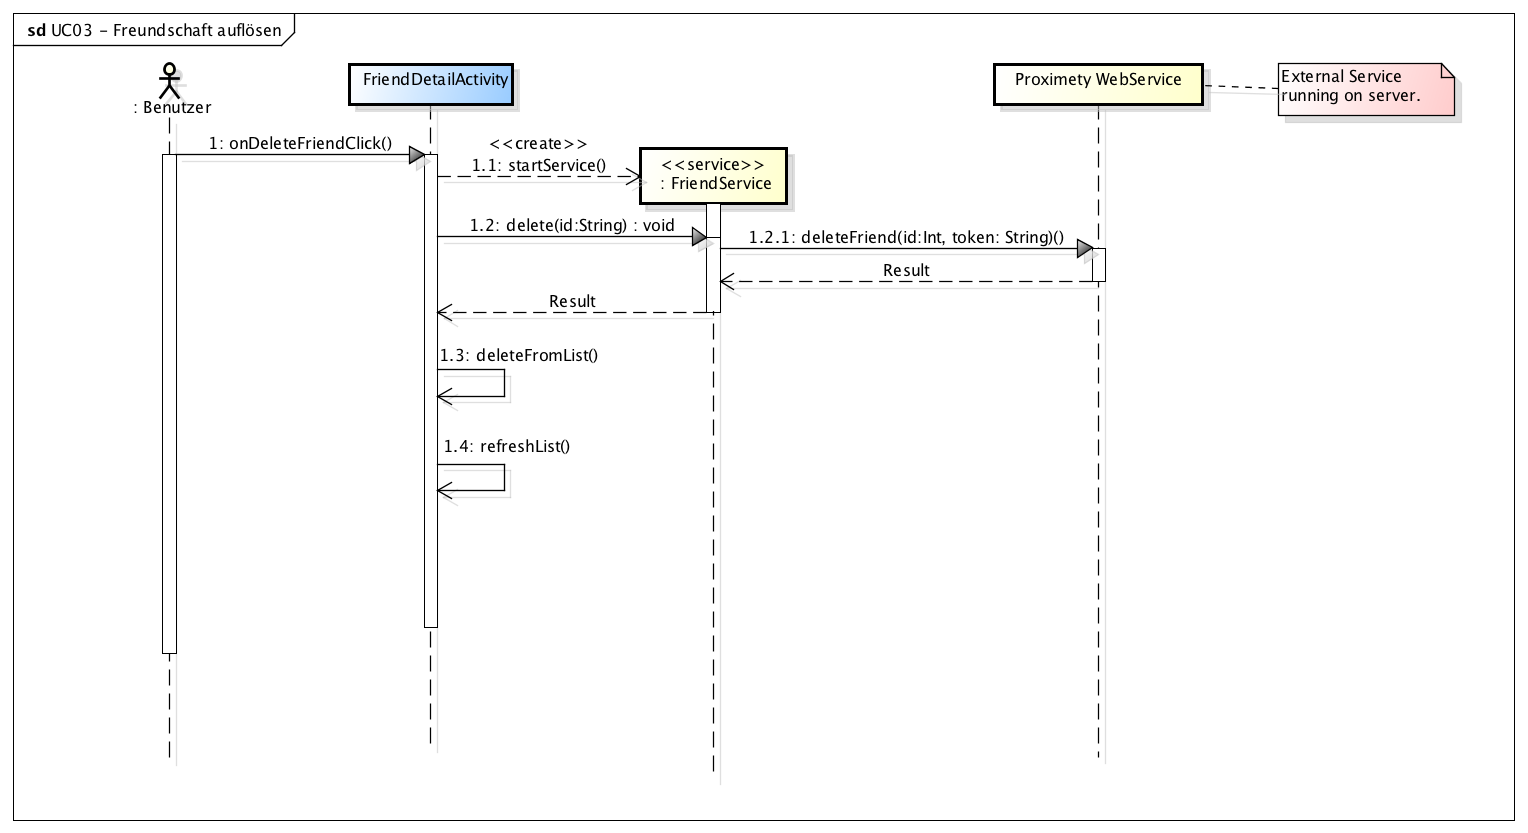
\includegraphics[width=\textwidth]{architektur/UC03_Freundschaft_aufloesen}
	\caption{Sequenzdiagramm Freundschaft aufloesen}
	\label{fig:UC03_Freundschaft_aufloesen}
\end{figure}
\FloatBarrier



\pagebreak
\subsubsection{Sequenzdiagramm Aktueller Standort eines Freundes abfragen}
\begin{figure}[H]
	\centering
		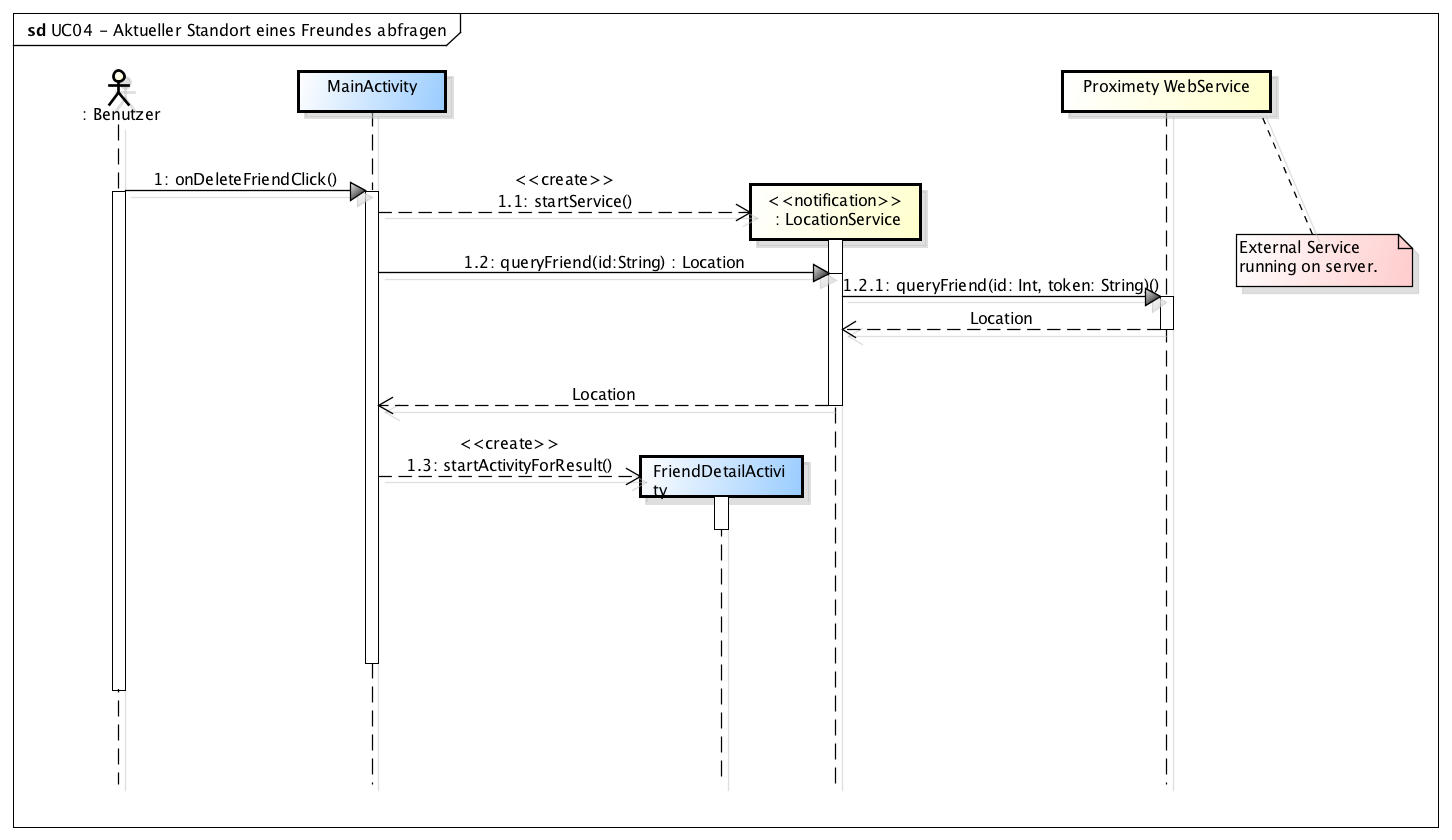
\includegraphics[width=\textwidth]{architektur/UC04_Aktueller_Standort_eines_Freundes_abfragen}
	\caption{Sequenzdiagramm Aktueller Standort eines Freundes abfragen}
	\label{fig:UC04_Aktueller_Standort_eines_Freundes_abfragen}
\end{figure}
\FloatBarrier



\pagebreak
\subsubsection{Sequenzdiagramm Proximety Alarm}
\begin{figure}[H]
	\centering
		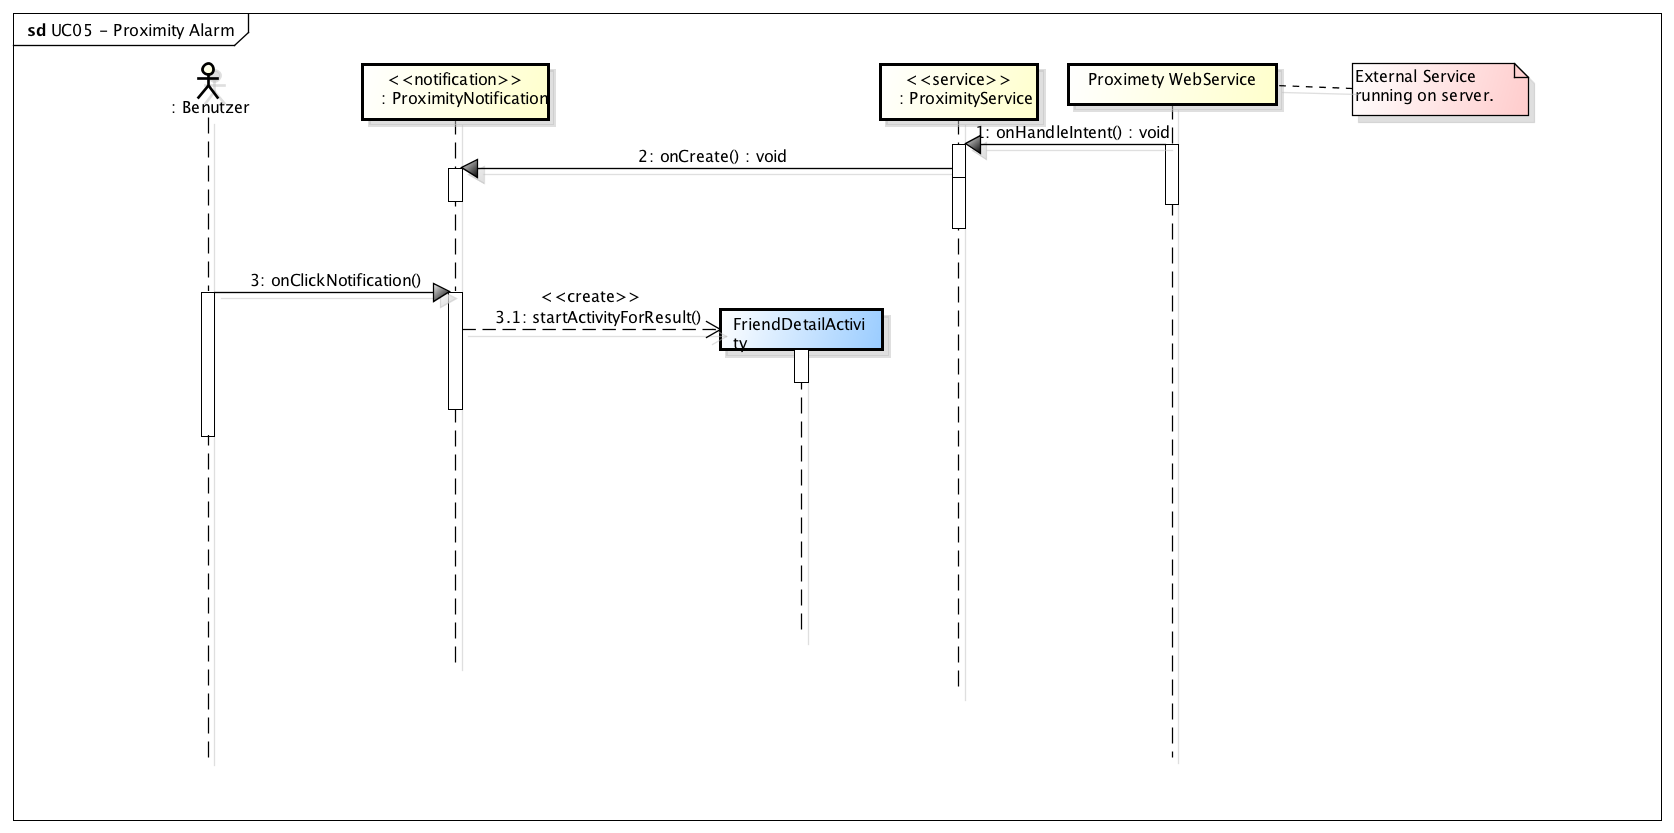
\includegraphics[width=\textwidth]{architektur/UC05_Proximity_Alarm}
	\caption{Sequenzdiagramm Proximety Alarm}
	\label{fig:UC05_Proximity_Alarm}
\end{figure}
\FloatBarrier



\pagebreak
\subsubsection{Sequenzdiagramm Freund kontaktieren}
\begin{figure}[H]
	\centering
		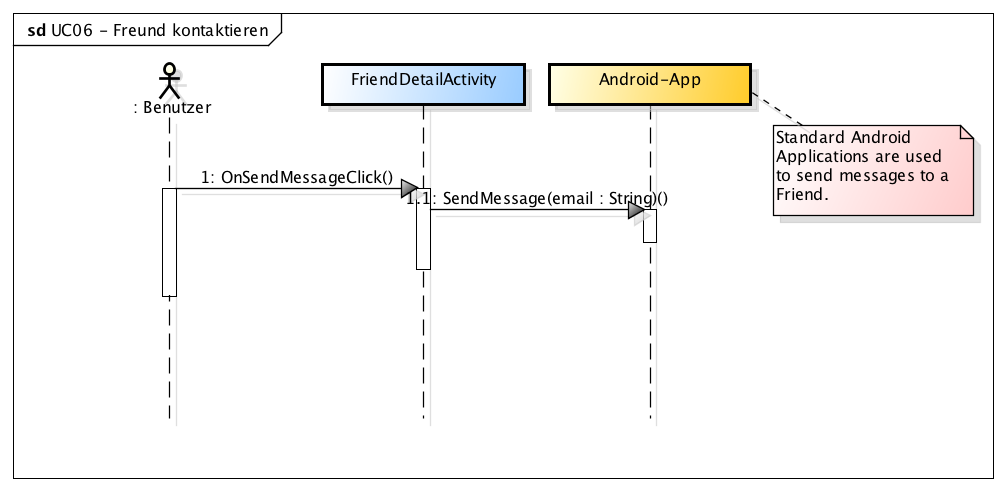
\includegraphics[width=\textwidth]{architektur/UC06_Freund_kontaktieren}
	\caption{Sequenzdiagramm Freund kontaktieren}
	\label{fig:UC06_Freund_kontaktieren}
\end{figure}
\FloatBarrier



\pagebreak
\subsubsection{Sequenzdiagramm Freundspezifische Einstellungen anpassen}
\begin{figure}[H]
	\centering
		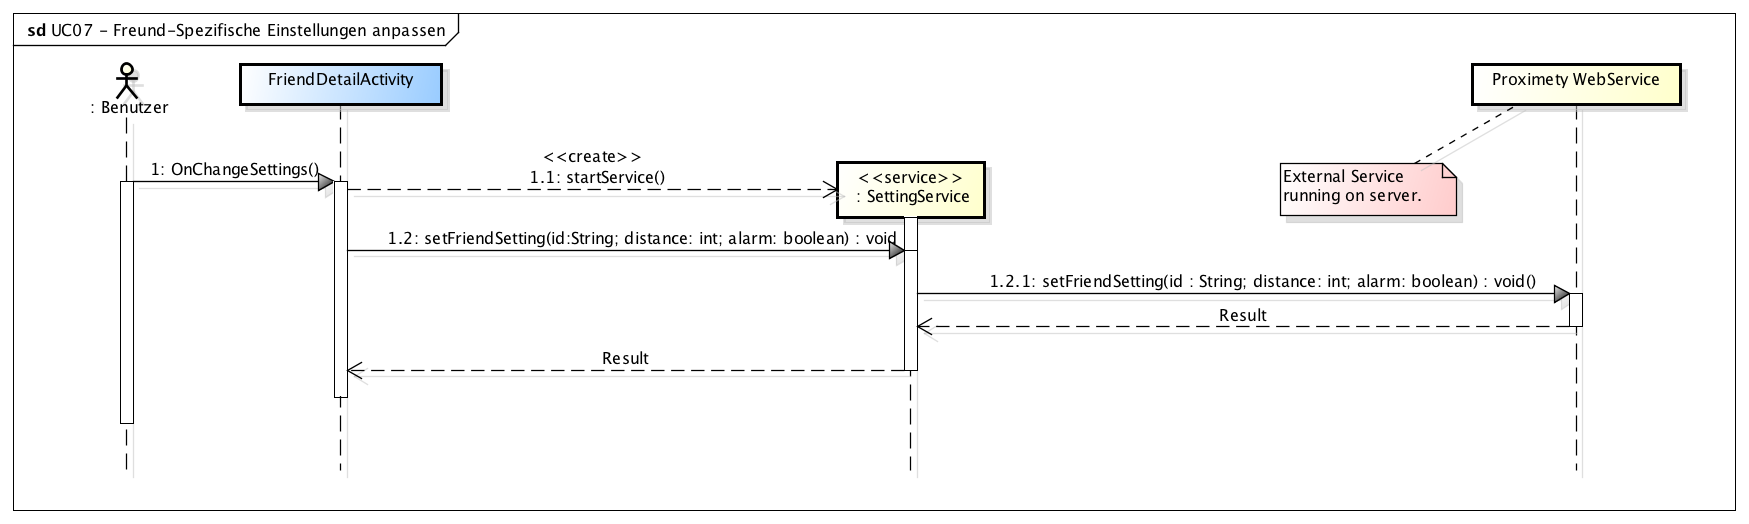
\includegraphics[width=\textwidth]{architektur/UC07_Freund_Spezifische_Einstellungen_anpassen}
	\caption{Sequenzdiagramm Freundspezifische Einstellungen anpassen}
	\label{fig:UC07_Freund_Spezifische_Einstellungen_anpassen}
\end{figure}
\FloatBarrier



\pagebreak
\subsubsection{Sequenzdiagramm Allgemeine App-Einstellungen vornehmen}
\begin{figure}[H]
	\centering
		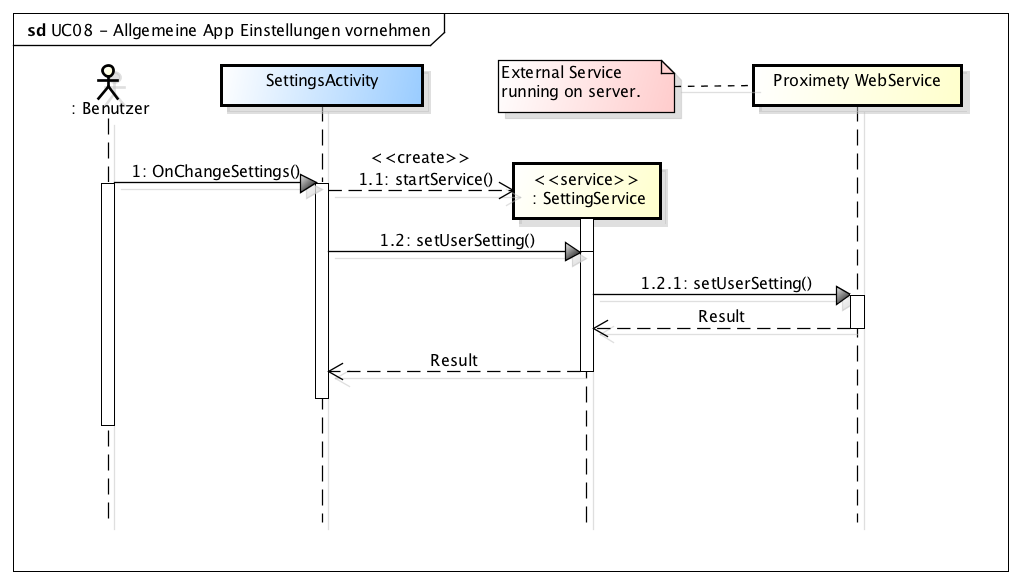
\includegraphics[width=\textwidth]{architektur/UC08_Allgemeine_App_Einstellungen_vornehmen}
	\caption{Sequenzdiagramm Allgemeine App-Einstellungen vornehmen}
	\label{fig:UC08_Allgemeine_App_Einstellungen_vornehmen}
\end{figure}
\FloatBarrier

%--- Appendix -------------------
\newpage
\appendix
\listoffigures
\listoftables

%-- Import Literature ----
\newpage
\renewcommand{\refname}{Quellenverzeichnis} 
\bibliography{allgemein/literatur}
\bibliographystyle{alpha}
\end{document}
